\section{Lựa chọn Thiết bị và Dự toán Chi phí (BOM)}

\subsection{Tiêu chí lựa chọn phần cứng}
Với ngân sách giới hạn \textbf{1.000.000.000 VNĐ} (Một tỷ đồng), việc sử dụng hoàn toàn các dòng thiết bị Enterprise cao cấp (như Cisco Catalyst 9000 Series) là không khả thi. Do đó, nhóm thiết kế quyết định chiến lược "Mix-Vendor" (Kết hợp đa hãng) để tối ưu hóa chi phí/hiệu năng:

\begin{itemize}
    \item \textbf{Firewall (Ưu tiên An ninh):} Sử dụng \textbf{Fortinet}. Đây là hãng dẫn đầu về hiệu năng/giá thành (Price/Performance) và tính năng bảo mật (NGFW).
    \item \textbf{Switching (Ưu tiên Sẵn sàng):} Sử dụng dòng \textbf{Cisco CBS (Business Series)} hoặc \textbf{Ruijie Enterprise}. Đảm bảo tính ổn định L2/L3 nhưng giá rẻ hơn dòng Catalyst 50\%.
    \item \textbf{Wireless (Wifi):} Sử dụng \textbf{Aruba Instant On}. Dễ quản lý qua Cloud, chịu tải tốt cho môi trường giáo dục.
\end{itemize}

\subsection{Danh mục Thiết bị và Báo giá Dự kiến}
Dưới đây là bảng dự toán chi tiết (Bill of Materials) cho Cơ sở Bảo Lộc:

\begin{table}[H]
\centering
\begin{tabularx}{\linewidth}{|c|l|X|c|r|r|}
\hline
\textbf{STT} & \textbf{Hạng mục} & \textbf{Model Đề xuất} & \textbf{SL} & \textbf{Đơn giá (VNĐ)} & \textbf{Thành tiền} \\ \hline
\rowcolor[HTML]{EFEFEF} 
\multicolumn{6}{|l|}{\textbf{A. HỆ THỐNG LÕI \& BẢO MẬT (CORE \& SECURITY)}} \\ \hline
1 & Firewall NGFW & \textbf{FortiGate 100F} (Kèm License 1 năm) & 01 & 80.000.000 & 80.000.000 \\ \hline
2 & Core Switch L3 & \textbf{Ruijie RG-S5750-24GT} (Dự phòng HA) & 02 & 35.000.000 & 70.000.000 \\ \hline
\rowcolor[HTML]{EFEFEF} 
\multicolumn{6}{|l|}{\textbf{B. HỆ THỐNG TRUY CẬP (DISTRIBUTION \& ACCESS)}} \\ \hline
3 & Dist Switch & \textbf{Ruijie RG-S2910-24GT4XS-E} & 02 & 15.000.000 & 30.000.000 \\ \hline
4 & Access Switch & \textbf{Ruijie RG-S2910-48GT4XS-P-E} (PoE+) & 10 & 25.000.000 & 250.000.000 \\ \hline
5 & Wifi 6 AP & \textbf{Aruba Instant On AP22} & 30 & 4.500.000 & 135.000.000 \\ \hline
\rowcolor[HTML]{EFEFEF} 
\multicolumn{6}{|l|}{\textbf{C. HẠ TẦNG \& PHỤ KIỆN}} \\ \hline
6 & Cabling & Cáp mạng CAT6 (Commscope) + Patch panel & 01 & 150.000.000 & 150.000.000 \\ \hline
7 & Labor & Nhân công triển khai & 01 & 100.000.000 & 100.000.000 \\ \hline
8 & Contingency & Chi phí dự phòng phí (10\%) & 01 & 81.500.000 & 81.500.000 \\ \hline
\multicolumn{5}{|r|}{\textbf{TỔNG CỘNG (Đã bao gồm VAT):}} & \textbf{896.500.000} \\ \hline
\end{tabularx}
\caption{Bảng dự toán kinh phí triển khai (Dự kiến)}
\label{tab:bom}
\end{table}

\subsection{Phân tích Đánh đổi (Trade-off Analysis)}
Trong quá trình lập dự toán, nhóm đã thực hiện so sánh giữa Phương án A (Lý tưởng) và Phương án B (Tối ưu) để đáp ứng yêu cầu ngân sách.

\begin{figure}[H]
    \centering
    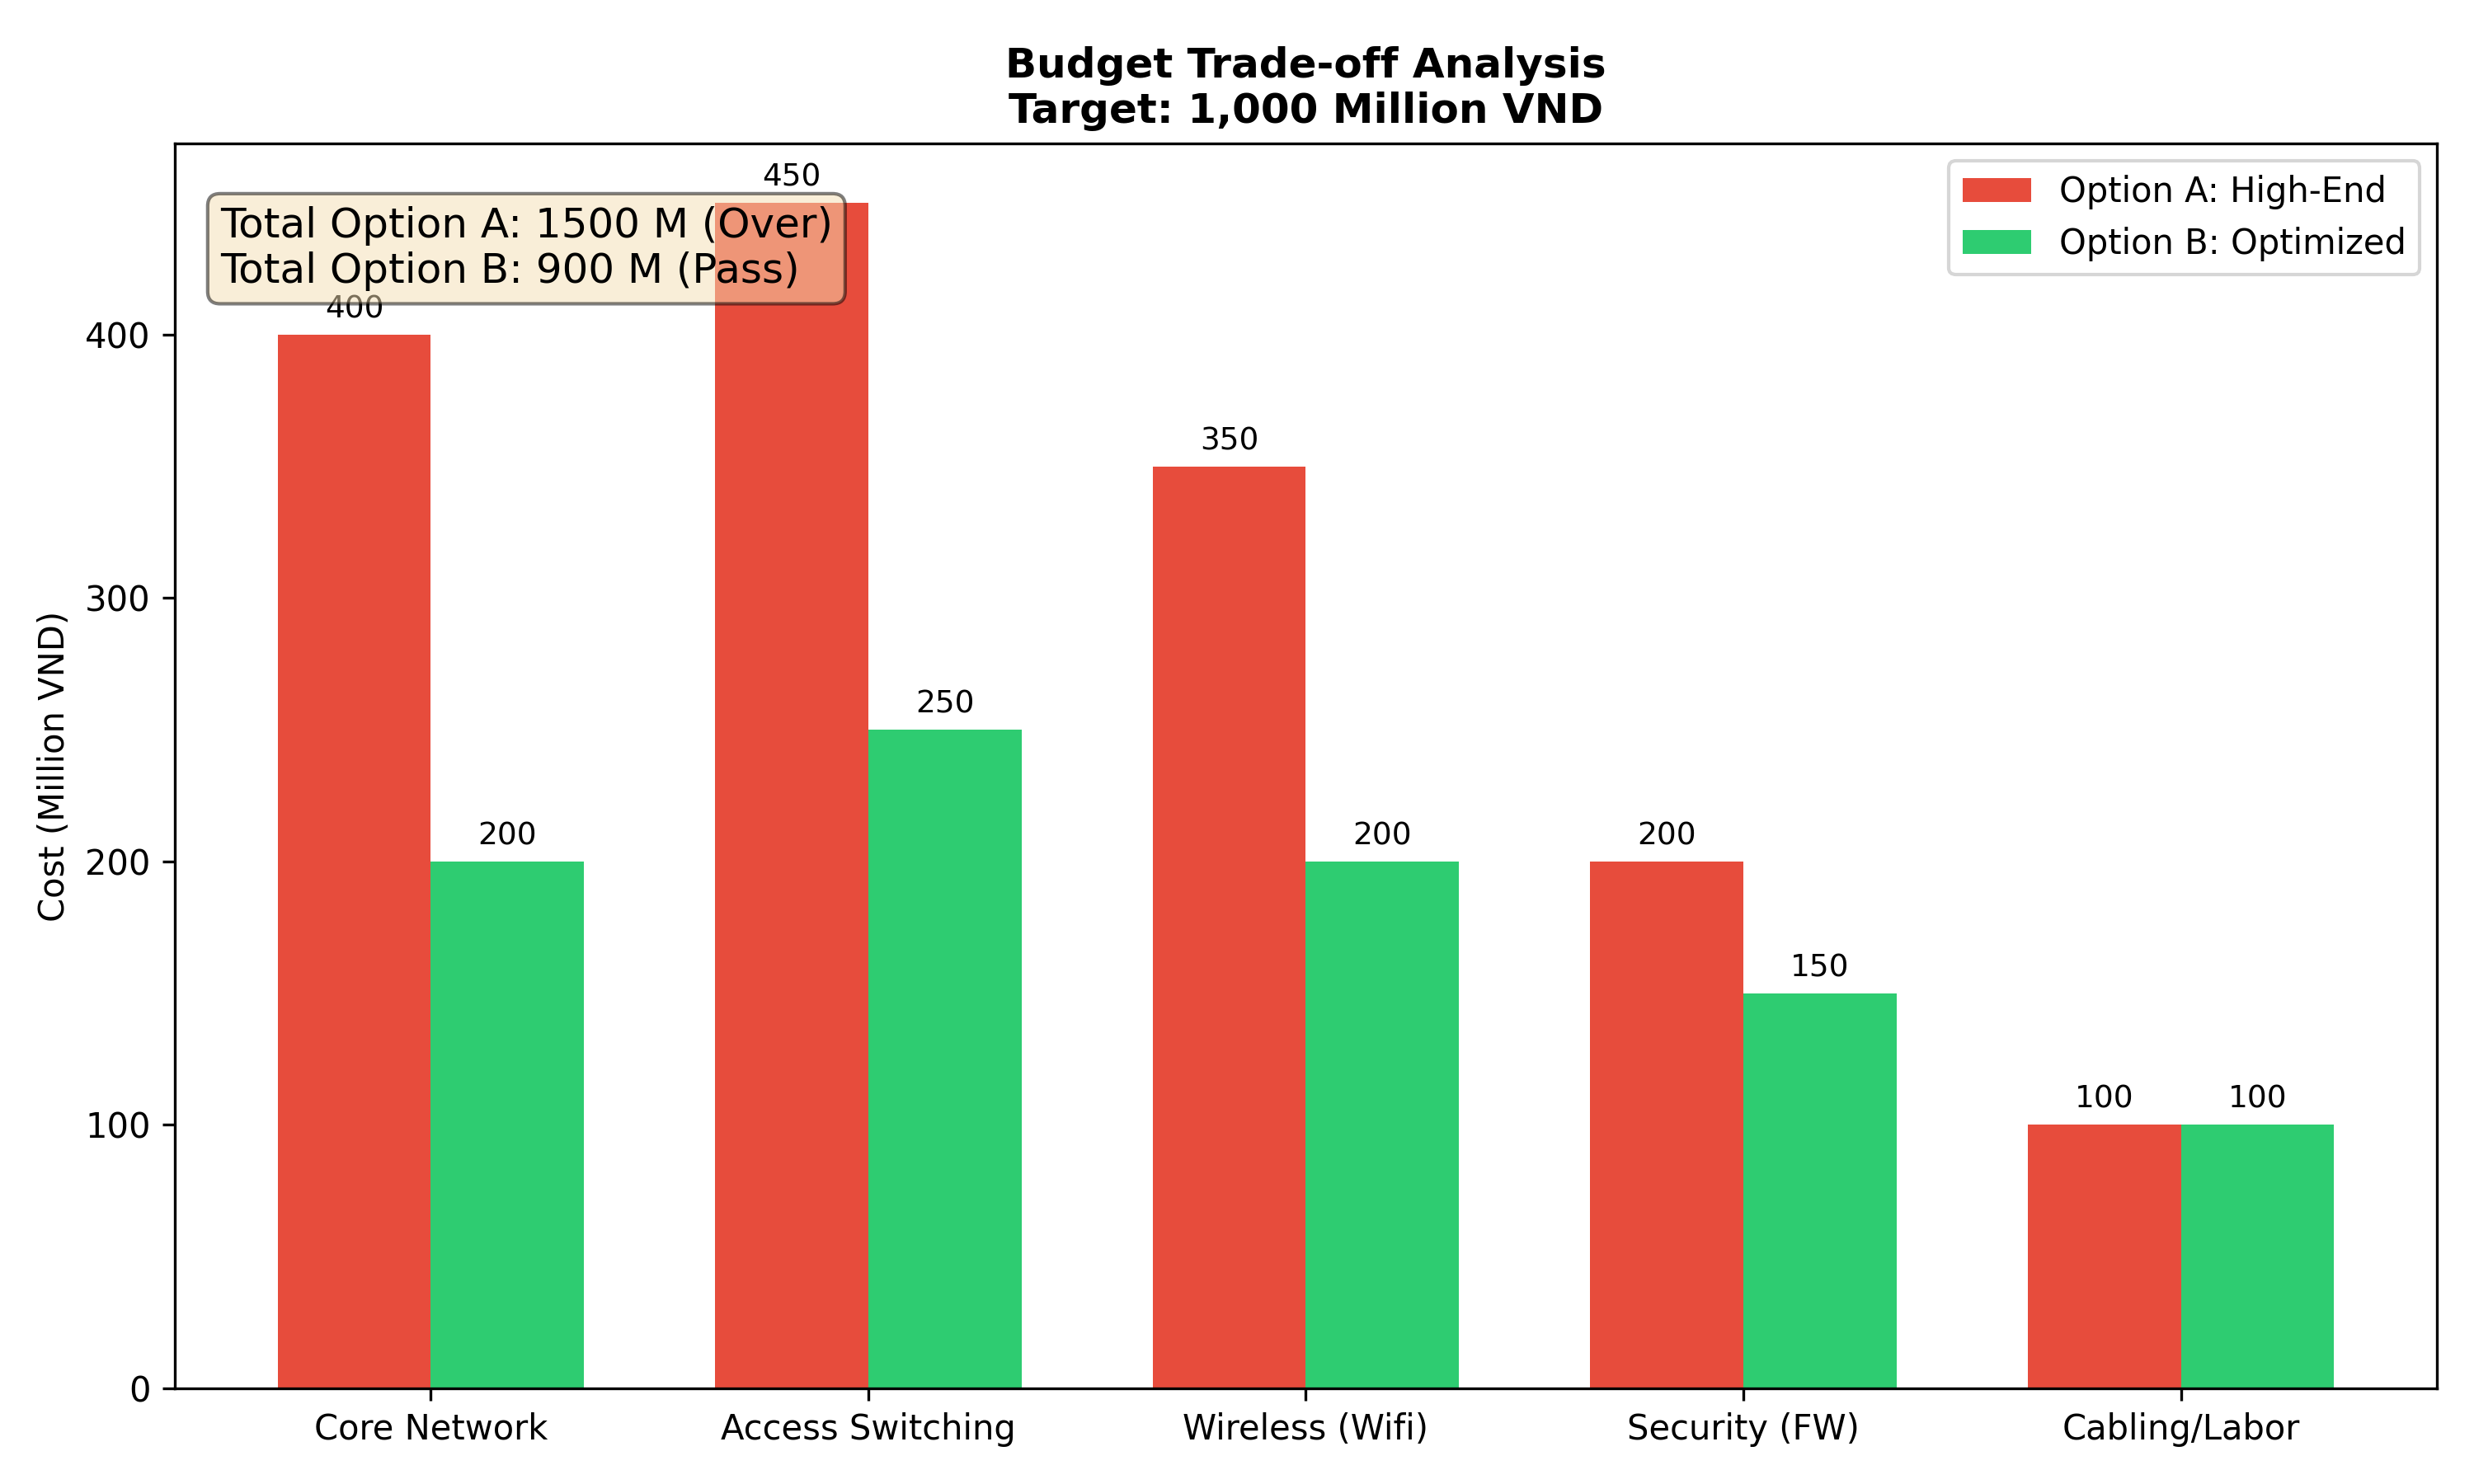
\includegraphics[width=0.8\linewidth]{image/budget_tradeoff.png}
    \caption{So sánh ngân sách giữa phương án High-end và Tối ưu}
    \label{fig:budget_chart}
\end{figure}

\textbf{Quyết định đánh đổi cụ thể:}
\begin{enumerate}
    \item \textbf{Thay thế Cisco Catalyst bằng Ruijie/Cisco CBS:}
    \begin{itemize}
        \item \textit{Được:} Giảm chi phí thiết bị chuyển mạch từ 800 triệu xuống còn 350 triệu.
        \item \textit{Mất:} Mất một số tính năng chuyên sâu của Cisco DNA Center (nhưng không quá cần thiết cho quy mô chi nhánh Bảo Lộc).
    \end{itemize}
    
    \item \textbf{Giữ nguyên Firewall FortiGate 100F:}
    \begin{itemize}
        \item Mặc dù đắt đỏ, nhưng nhóm quyết định \textbf{không cắt giảm} chi phí bảo mật. Lý do dựa trên Bảng trọng số (Mục 1) xác định "An ninh" là ưu tiên hàng đầu (20\%).
    \end{itemize}
    
    \item \textbf{Giảm số lượng AP dự phòng:}
    \begin{itemize}
        \item Giảm mật độ phủ sóng từ "Dày đặc" xuống "Tiêu chuẩn" để tiết kiệm chi phí mua Access Point.
    \end{itemize}
\end{enumerate}

\textbf{Kết luận tài chính:} Với tổng chi phí dự kiến là \textbf{896.500.000 VNĐ}, dự án nằm trong ngưỡng an toàn (< 1 tỷ VNĐ) và vẫn còn khoảng 100 triệu dự phòng cho các phát sinh thực tế.